\documentclass{standalone}
\usepackage{tikz}
\usetikzlibrary{patterns, positioning}
\usepackage[sfdefault]{ClearSans} %% option 'sfdefault' activates Clear Sans as the default text font
\usepackage[T1]{fontenc}

\begin{document}
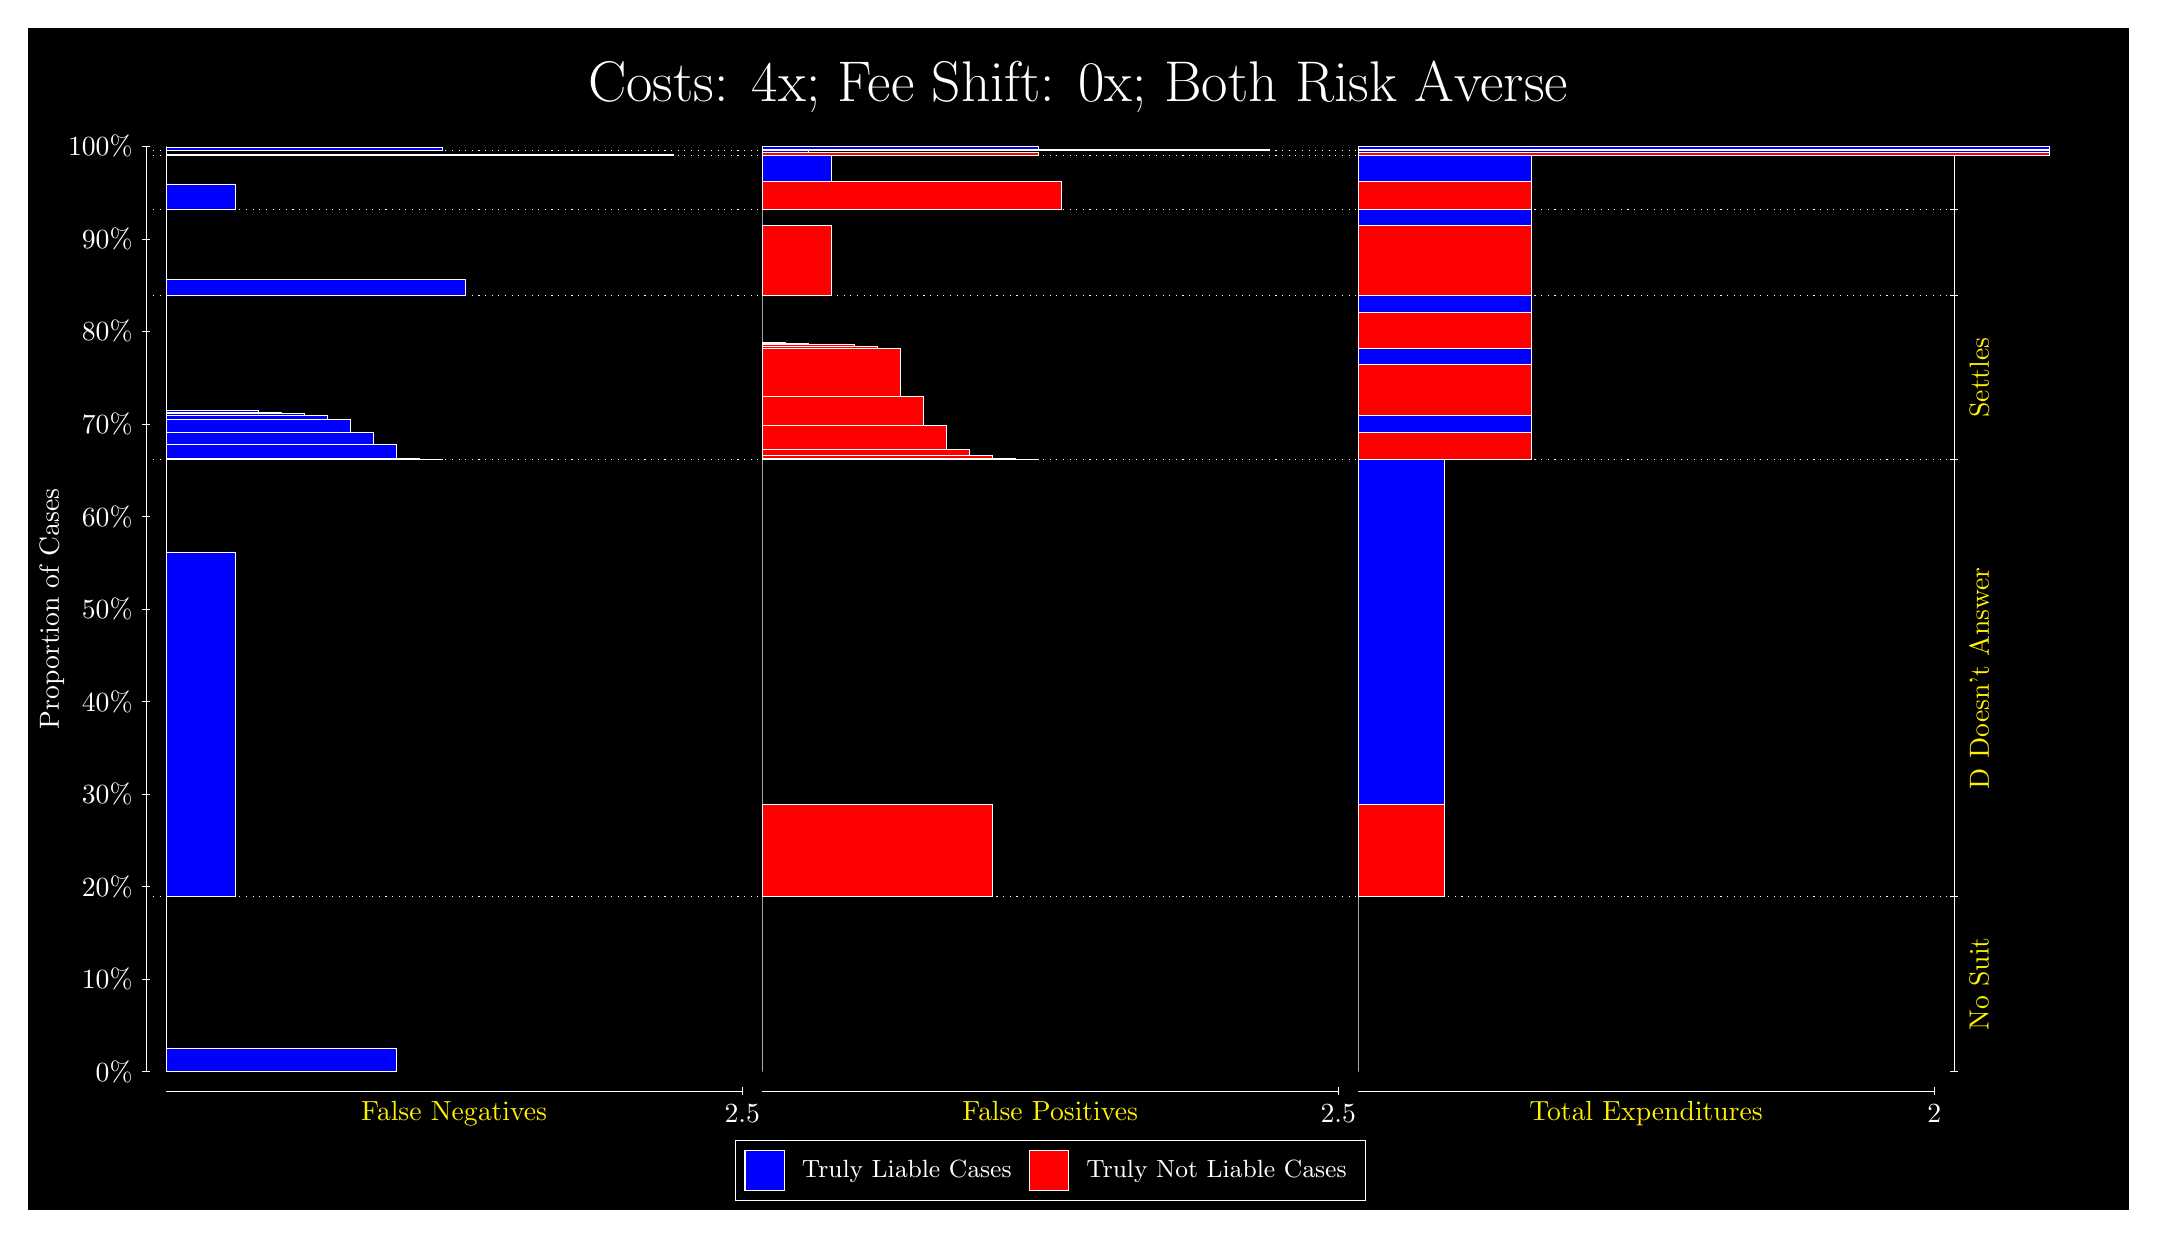
\begin{tikzpicture}
\draw[fill=black] (0,0) rectangle (26.667,15);
\draw[text=white] (0,13.5) rectangle (26.667,15) node[midway] {\huge Costs: 4x; Fee Shift: 0x; Both Risk Averse};
\draw[white, very thin] (1.5,1.75) -- (1.5,13.5);
\node[rotate=90, text=white, anchor=center] at (0.3, 7.625) {Proportion of Cases};
\draw[white, very thin] (1.45,1.75) -- (1.55,1.75);
\node[text=white, anchor=east] at (1.45, 1.75) {0\%};
\draw[white, very thin] (1.45,2.925) -- (1.55,2.925);
\node[text=white, anchor=east] at (1.45, 2.925) {10\%};
\draw[white, very thin] (1.45,4.1) -- (1.55,4.1);
\node[text=white, anchor=east] at (1.45, 4.1) {20\%};
\draw[white, very thin] (1.45,5.275) -- (1.55,5.275);
\node[text=white, anchor=east] at (1.45, 5.275) {30\%};
\draw[white, very thin] (1.45,6.45) -- (1.55,6.45);
\node[text=white, anchor=east] at (1.45, 6.45) {40\%};
\draw[white, very thin] (1.45,7.625) -- (1.55,7.625);
\node[text=white, anchor=east] at (1.45, 7.625) {50\%};
\draw[white, very thin] (1.45,8.8) -- (1.55,8.8);
\node[text=white, anchor=east] at (1.45, 8.8) {60\%};
\draw[white, very thin] (1.45,9.975) -- (1.55,9.975);
\node[text=white, anchor=east] at (1.45, 9.975) {70\%};
\draw[white, very thin] (1.45,11.15) -- (1.55,11.15);
\node[text=white, anchor=east] at (1.45, 11.15) {80\%};
\draw[white, very thin] (1.45,12.325) -- (1.55,12.325);
\node[text=white, anchor=east] at (1.45, 12.325) {90\%};
\draw[white, very thin] (1.45,13.5) -- (1.55,13.5);
\node[text=white, anchor=east] at (1.45, 13.5) {100\%};

\draw[white, very thin] (24.457,1.75) -- (24.457,13.5);
\draw[white, very thin] (24.407,1.75) -- (24.507,1.75);
\node[anchor=west] at (24.407, 1.75) {};
\draw[white, very thin] (24.407,3.9727) -- (24.507,3.9727);
\node[anchor=west] at (24.407, 3.9727) {};
\draw[white, very thin] (24.407,9.5194) -- (24.507,9.5194);
\node[anchor=west] at (24.407, 9.5194) {};
\draw[white, very thin] (24.407,11.608) -- (24.507,11.608);
\node[anchor=west] at (24.407, 11.608) {};
\draw[white, very thin] (24.407,12.696) -- (24.507,12.696);
\node[anchor=west] at (24.407, 12.696) {};
\draw[white, very thin] (24.407,13.388) -- (24.507,13.388);
\node[anchor=west] at (24.407, 13.388) {};
\draw[white, very thin] (24.407,13.444) -- (24.507,13.444);
\node[anchor=west] at (24.407, 13.444) {};
\draw[white, very thin] (24.407,13.5) -- (24.507,13.5);
\node[anchor=west] at (24.407, 13.5) {};

\draw[white, very thin, fill=blue] (1.75,1.75) rectangle (4.6775,2.0421);
\draw[white, very thin, fill=red] (1.75,2.0421) rectangle (1.75,3.9727);
\draw[white, very thin, fill=blue] (1.75,3.9727) rectangle (2.6283,8.3439);
\draw[white, very thin, fill=red] (1.75,8.3439) rectangle (1.75,9.5194);
\draw[white, very thin, fill=blue] (1.75,9.5194) rectangle (5.2631,9.5247);
\draw[white, very thin, fill=blue] (1.75,9.5247) rectangle (4.9703,9.5373);
\draw[white, very thin, fill=blue] (1.75,9.5373) rectangle (4.6775,9.7125);
\draw[white, very thin, fill=blue] (1.75,9.7125) rectangle (4.3848,9.7153);
\draw[white, very thin, fill=blue] (1.75,9.7153) rectangle (4.3848,9.8687);
\draw[white, very thin, fill=blue] (1.75,9.8687) rectangle (4.092,10.033);
\draw[white, very thin, fill=blue] (1.75,10.033) rectangle (3.7993,10.08);
\draw[white, very thin, fill=blue] (1.75,10.08) rectangle (3.5065,10.115);
\draw[white, very thin, fill=blue] (1.75,10.115) rectangle (3.2138,10.127);
\draw[white, very thin, fill=blue] (1.75,10.127) rectangle (2.921,10.145);
\draw[white, very thin, fill=red] (1.75,10.145) rectangle (1.75,11.608);
\draw[white, very thin, fill=blue] (1.75,11.608) rectangle (5.5558,11.811);
\draw[white, very thin, fill=red] (1.75,11.811) rectangle (1.75,12.696);
\draw[white, very thin, fill=blue] (1.75,12.696) rectangle (2.6283,13.023);
\draw[white, very thin, fill=red] (1.75,13.023) rectangle (1.75,13.388);
\draw[white, very thin, fill=blue] (1.75,13.388) rectangle (8.1906,13.403);
\draw[white, very thin, fill=red] (1.75,13.403) rectangle (1.75,13.444);
\draw[white, very thin, fill=blue] (1.75,13.444) rectangle (5.2631,13.485);
\draw[white, very thin, fill=red] (1.75,13.485) rectangle (1.75,13.5);
\draw[white, very thin, fill=red] (9.3189,1.75) rectangle (9.3189,3.6806);
\draw[white, very thin, fill=blue] (9.3189,3.6806) rectangle (9.3189,3.9727);
\draw[white, very thin, fill=red] (9.3189,3.9727) rectangle (12.246,5.1482);
\draw[white, very thin, fill=blue] (9.3189,5.1482) rectangle (9.3189,9.5194);
\draw[white, very thin, fill=red] (9.3189,9.5194) rectangle (12.832,9.5261);
\draw[white, very thin, fill=red] (9.3189,9.5261) rectangle (12.539,9.5319);
\draw[white, very thin, fill=red] (9.3189,9.5319) rectangle (12.246,9.572);
\draw[white, very thin, fill=red] (9.3189,9.572) rectangle (11.954,9.6549);
\draw[white, very thin, fill=red] (9.3189,9.6549) rectangle (11.661,9.9574);
\draw[white, very thin, fill=red] (9.3189,9.9574) rectangle (11.368,10.329);
\draw[white, very thin, fill=red] (9.3189,10.329) rectangle (11.075,10.935);
\draw[white, very thin, fill=red] (9.3189,10.935) rectangle (10.783,10.963);
\draw[white, very thin, fill=red] (9.3189,10.963) rectangle (10.49,10.982);
\draw[white, very thin, fill=blue] (9.3189,10.982) rectangle (9.9044,11);
\draw[white, very thin, fill=blue] (9.3189,11) rectangle (9.6116,11.012);
\draw[white, very thin, fill=blue] (9.3189,11.012) rectangle (9.3189,11.608);
\draw[white, very thin, fill=red] (9.3189,11.608) rectangle (10.197,12.494);
\draw[white, very thin, fill=blue] (9.3189,12.494) rectangle (9.3189,12.696);
\draw[white, very thin, fill=red] (9.3189,12.696) rectangle (13.125,13.061);
\draw[white, very thin, fill=blue] (9.3189,13.061) rectangle (10.197,13.388);
\draw[white, very thin, fill=red] (9.3189,13.388) rectangle (12.832,13.43);
\draw[white, very thin, fill=blue] (9.3189,13.43) rectangle (9.9044,13.444);
\draw[white, very thin, fill=red] (9.3189,13.444) rectangle (15.759,13.459);
\draw[white, very thin, fill=blue] (9.3189,13.459) rectangle (12.832,13.5);
\draw[white, very thin, fill=red] (16.888,1.75) rectangle (16.888,3.6806);
\draw[white, very thin, fill=blue] (16.888,3.6806) rectangle (16.888,3.9727);
\draw[white, very thin, fill=red] (16.888,3.9727) rectangle (17.986,5.1482);
\draw[white, very thin, fill=blue] (16.888,5.1482) rectangle (17.986,9.5194);
\draw[white, very thin, fill=red] (16.888,9.5194) rectangle (19.083,9.8677);
\draw[white, very thin, fill=blue] (16.888,9.8677) rectangle (19.083,10.079);
\draw[white, very thin, fill=red] (16.888,10.079) rectangle (19.083,10.735);
\draw[white, very thin, fill=blue] (16.888,10.735) rectangle (19.083,10.931);
\draw[white, very thin, fill=red] (16.888,10.931) rectangle (19.083,11.389);
\draw[white, very thin, fill=blue] (16.888,11.389) rectangle (19.083,11.608);
\draw[white, very thin, fill=red] (16.888,11.608) rectangle (19.083,12.494);
\draw[white, very thin, fill=blue] (16.888,12.494) rectangle (19.083,12.696);
\draw[white, very thin, fill=red] (16.888,12.696) rectangle (19.083,13.061);
\draw[white, very thin, fill=blue] (16.888,13.061) rectangle (19.083,13.388);
\draw[white, very thin, fill=red] (16.888,13.388) rectangle (25.67,13.43);
\draw[white, very thin, fill=blue] (16.888,13.43) rectangle (25.67,13.444);
\draw[white, very thin, fill=red] (16.888,13.444) rectangle (25.67,13.459);
\draw[white, very thin, fill=blue] (16.888,13.459) rectangle (25.67,13.5);
\draw[white, dotted] (1.5,3.9727) -- (24.457,3.9727);
\draw[white, dotted] (1.5,9.5194) -- (24.457,9.5194);
\draw[white, dotted] (1.5,11.608) -- (24.457,11.608);
\draw[white, dotted] (1.5,12.696) -- (24.457,12.696);
\draw[white, dotted] (1.5,13.388) -- (24.457,13.388);
\draw[white, dotted] (1.5,13.444) -- (24.457,13.444);
\draw[white, very thin] (1.75,1.5) -- (9.0689,1.5);
\node[text=yellow, anchor=north] at (5.4094, 1.5) {False Negatives};
\draw[white, very thin] (9.0689,1.45) -- (9.0689,1.55);
\node[text=white, anchor=north] at (9.0689, 1.45) {2.5};

\draw[white, very thin] (9.3189,1.5) -- (16.638,1.5);
\node[text=yellow, anchor=north] at (12.978, 1.5) {False Positives};
\draw[white, very thin] (16.638,1.45) -- (16.638,1.55);
\node[text=white, anchor=north] at (16.638, 1.45) {2.5};

\draw[white, very thin] (16.888,1.5) -- (24.207,1.5);
\node[text=yellow, anchor=north] at (20.547, 1.5) {Total Expenditures};
\draw[white, very thin] (24.207,1.45) -- (24.207,1.55);
\node[text=white, anchor=north] at (24.207, 1.45) {2};

\node[text=yellow, centered, rotate=90] at (24.777, 2.8613) {No Suit};
\node[text=yellow, centered, rotate=90] at (24.777, 6.7461) {D Doesn't Answer};
\node[text=yellow, centered, rotate=90] at (24.777, 10.564) {Settles};





\draw (12.978300999999998,1.5) node[draw=none] (baseCoordinate) {};
\begin{scope}[align=center]
        \matrix[scale=0.5, draw=white, below=0.5cm of baseCoordinate, nodes={draw}, column sep=0.1cm]{
            \node[rectangle, draw, minimum width=0.5cm, minimum height=0.5cm, fill=blue] {}; &
            \node[draw=none, font=\small, text=white] (B) {Truly Liable Cases}; &
            \node[rectangle, draw, minimum width=0.5cm, minimum height=0.5cm, fill=red] {}; &
            \node[draw=none, font=\small, text=white] (B) {Truly Not Liable Cases}; \\
            };
\end{scope}

\end{tikzpicture}
\end{document}